\section{Matched text-to-image CFG sweeps}

The text-to-image runs evaluate latent-diffusion models
\citep{rombach2022ldm} with the Diffusers Euler solver, NFE 10, seeds 0, 1,
and 2, and 50 prompts from \texttt{diffusers\_ablation\_prompts}. Each base,
published AYS \citep{sabour2024ays}, and our row is matched by prompt, seed,
model, solver, NFE, and guidance scale. The metrics are CLIPScore
\citep{hessel2022clipscore,radford2021clip} and ImageReward
\citep{xu2023imagereward}, where higher is better.

\subsection{Stable Diffusion 1.5}

The SD1.5 sweep uses guidance scales 5.0, 7.5, and 10.0. It retains the
largest text-to-image calibration setting in this draft, with 9 calibrated
schedules and 1350 scored images.

\begin{figure}[t]
  \centering
  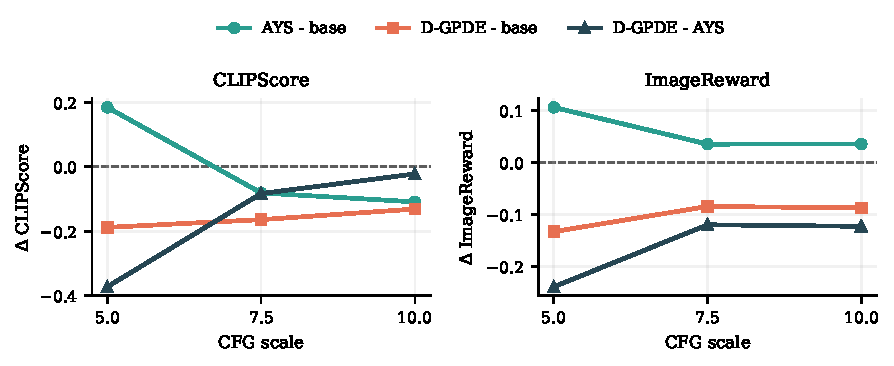
\includegraphics[width=0.86\linewidth]{figures/sd15_euler_nfe10_cfg_sweep_pairwise.pdf}
  \caption{Matched SD1.5 text-to-image pairwise mean deltas for model
  \texttt{stable\_diffusion\_15}, Diffusers Euler solver, NFE 10, guidance
  scales 5.0, 7.5, and 10.0, schedules base, AYS, and ours, seeds 0--2,
  and 50 prompts per seed from \texttt{diffusers\_ablation\_prompts}. Deltas
  are computed over 150 matched prompt/seed pairs per guidance scale. CLIPScore
  and ImageReward are higher-is-better.}
  \label{fig:sd15-euler-nfe10-cfg-sweep-pairwise}
\end{figure}

\begin{table}[t]
  \centering
  \caption{SD1.5 text-to-image matched CFG sweep with Euler solver,
  NFE 10, seeds 0--2, and 50 prompts from
  \texttt{diffusers\_ablation\_prompts}. Rows report pairwise mean
  deltas and win rates over 150 matched prompt/seed pairs. CLIPScore
  and ImageReward are higher-is-better.}
  \label{tab:sd15-euler-nfe10-cfg-sweep-pairwise}
  \begin{tabular}{llrrrr}
    \toprule
    CFG & comparison & $\Delta$CLIP & CLIP win (\%) & $\Delta$IR & IR win (\%) \\
    \midrule
    5 & AYS - base & +0.18 & 53.3 & +0.106 & 66.0 \\
    5 & ours - base & -0.19 & 42.7 & -0.133 & 33.3 \\
    5 & ours - AYS & -0.37 & 41.3 & -0.239 & 26.7 \\
    7.5 & AYS - base & -0.08 & 51.3 & +0.035 & 57.3 \\
    7.5 & ours - base & -0.16 & 45.3 & -0.084 & 46.0 \\
    7.5 & ours - AYS & -0.08 & 47.3 & -0.120 & 38.7 \\
    10 & AYS - base & -0.11 & 46.0 & +0.035 & 54.0 \\
    10 & ours - base & -0.13 & 41.3 & -0.087 & 40.7 \\
    10 & ours - AYS & -0.02 & 48.0 & -0.123 & 37.3 \\
    \bottomrule
  \end{tabular}
\end{table}


\subsection{SDXL}

The SDXL sweep \citep{podell2023sdxl} uses guidance scales 5.0 and 7.5. It
uses a lighter calibration configuration than SD1.5: one prompt per batch, four
calibration batches, 64 reference steps, a 65-node reference grid, and a
128-node candidate grid. This choice keeps the run within the minimum
validation budget while preserving the matched base/AYS/ours comparison
across three seeds.

\begin{figure}[t]
  \centering
  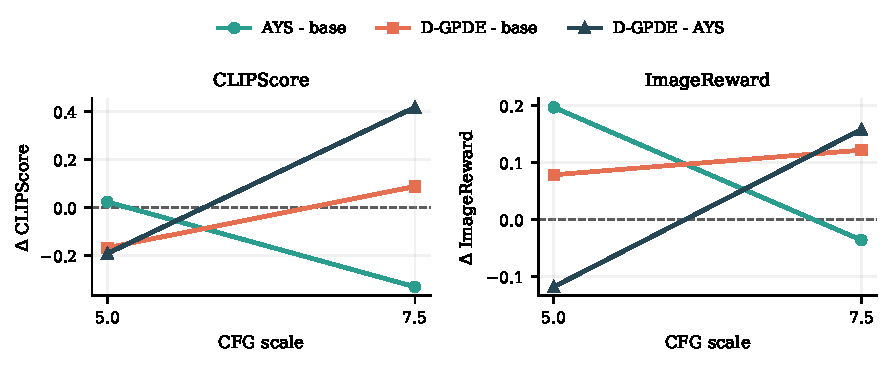
\includegraphics[width=0.86\linewidth]{figures/sdxl_euler_nfe10_cfg_sweep_pairwise.pdf}
  \caption{Matched SDXL text-to-image pairwise mean deltas for model
  \texttt{sdxl}, Diffusers Euler solver, NFE 10, guidance scales 5.0 and 7.5,
  schedules base, AYS, and ours, seeds 0--2, and 50 prompts per seed from
  \texttt{diffusers\_ablation\_prompts}. Deltas are computed over 150 matched
  prompt/seed pairs per guidance scale. CLIPScore and ImageReward are
  higher-is-better.}
  \label{fig:sdxl-euler-nfe10-cfg-sweep-pairwise}
\end{figure}

\begin{table}[t]
  \centering
  \caption{SDXL text-to-image matched CFG sweep with Euler solver,
  NFE 10, seeds 0--2, and 50 prompts from
  \texttt{diffusers\_ablation\_prompts}. Rows report pairwise mean
  deltas and win rates over 150 matched prompt/seed pairs. CLIPScore
  and ImageReward are higher-is-better.}
  \label{tab:sdxl-euler-nfe10-cfg-sweep-pairwise}
  \begin{tabular}{llrrrr}
    \toprule
    CFG & comparison & $\Delta$CLIP & CLIP win (\%) & $\Delta$IR & IR win (\%) \\
    \midrule
    5 & AYS - base & +0.02 & 46.0 & +0.197 & 66.0 \\
    5 & ours - base & -0.17 & 43.3 & +0.079 & 52.7 \\
    5 & ours - AYS & -0.19 & 48.0 & -0.119 & 35.3 \\
    7.5 & AYS - base & -0.33 & 44.7 & -0.036 & 49.3 \\
    7.5 & ours - base & +0.09 & 46.7 & +0.122 & 54.7 \\
    7.5 & ours - AYS & +0.42 & 58.0 & +0.158 & 52.7 \\
    \bottomrule
  \end{tabular}
\end{table}


The SDXL result is condition-dependent. At CFG 5.0, our schedule improves
ImageReward over base by 0.079 but trails AYS by 0.119. At CFG 7.5, it improves
the mean CLIPScore and ImageReward deltas over both base and AYS. This pattern
supports condition-aware evaluation coverage and keeps the text-to-image claim
bounded to matched automated metrics.

\subsection{SD1.5 reuse and schedule diagnostics}

\begin{table}[t]
  \centering
  \caption{Actual SD1.5 schedule reuse check. We reuse a single
  our schedule calibrated at CFG 7.5, seed 0 for CFG 5.0, 7.5,
  and 10.0, seeds 0--2, and 50 prompts per seed. Rows report matched prompt/seed
  deltas for reuse minus the CFG- and seed-specific schedule.
  Higher is better for both metrics.}
  \label{tab:sd15-euler-nfe10-reuse-cfg7p5-seed0}
  \begin{tabular}{rrrrr}
    \toprule
    CFG & $\Delta$ CLIP & CLIP win (\%) & $\Delta$ ImageReward & IR win (\%) \\
    \midrule
    5 & -0.10 & 46.7 & +0.006 & 50.7 \\
    7.5 & -0.05 & 28.0 & +0.003 & 31.3 \\
    10 & -0.00 & 48.7 & +0.034 & 53.3 \\
    \bottomrule
  \end{tabular}
\end{table}


Table~\ref{tab:sd15-euler-nfe10-reuse-cfg7p5-seed0} reports a second actual
reuse check. We reuse the CFG 7.5, seed-0 schedule for CFG 5.0, 7.5,
and 10.0, seeds 0--2, with the same 50 prompts. Reuse stays near the CFG- and
seed-specific rows on ImageReward, with matched deltas from +0.003
to +0.034, but loses CLIPScore by up to 0.10. Against base and AYS, reuse
remains negative on both automated metrics in the pairwise summaries. The
result broadens reuse evidence while preserving the text-to-image conclusion as
mixed or negative.

Figure~\ref{fig:sd15-euler-nfe10-cfg7p5-schedule-profile} shows the sigma-grid
diagnostic for the CFG 7.5, seed-0 schedule bundle. Our schedule keeps
larger sigma values for more early boundaries than both base and AYS in this
representative case. This diagnostic explains allocation only; the quality
metrics below remain the evidence for the mixed result.

\begin{figure}[t]
  \centering
  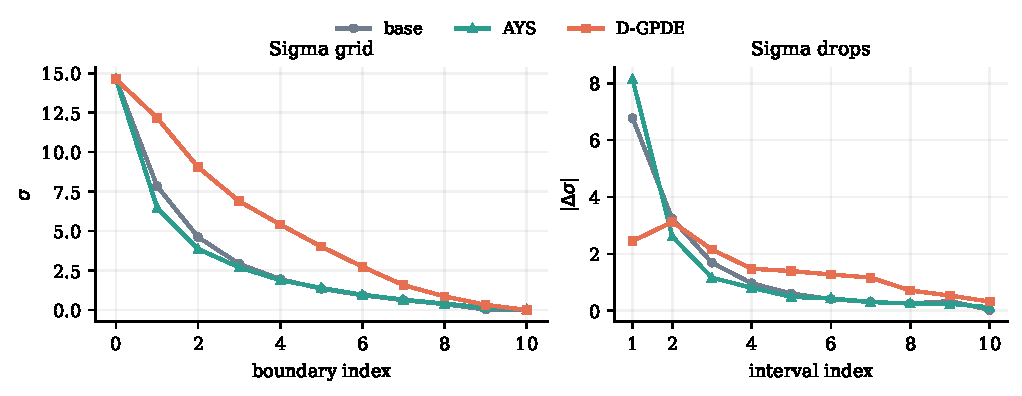
\includegraphics[width=0.82\linewidth]{figures/sd15_euler_nfe10_cfg7p5_schedule_profile_seed0.pdf}
  \caption{Stable Diffusion 1.5 Diffusers Euler NFE-10 schedule profile for
  guidance scale 7.5 and seed 0. The left panel shows the sigma grid for base,
  published AYS, and our schedules. The right panel shows sigma drops
  between adjacent boundaries. This is a schedule diagnostic, not a perceptual
  quality metric.}
  \label{fig:sd15-euler-nfe10-cfg7p5-schedule-profile}
\end{figure}

The SD1.5 sweep is a retained mixed result. AYS improves ImageReward over base
at all three guidance scales, while ours trails base and AYS on ImageReward and
underperforms base on CLIPScore under this SD1.5/Euler/NFE-10 setup. This
evidence supports a bounded failure analysis and CFG-matched evaluation
coverage. Cleaned rows, pairwise summaries, copied schedules, and oracle-reuse
cost accounting are stored under \texttt{paper/results/t2i/}. The same
directory includes the prompt manifest and prompt-index CSV for
\texttt{diffusers\_ablation\_prompts}. The source output roots are
\texttt{outputs/gpde\_diffusers\_sd15\_nfe10\_cfg\_seed\_sweep/} and
\texttt{outputs/gpde\_diffusers\_sdxl\_nfe10\_cfg\_seed\_sweep/}.
